\begin{figure}[t]
    \centering
    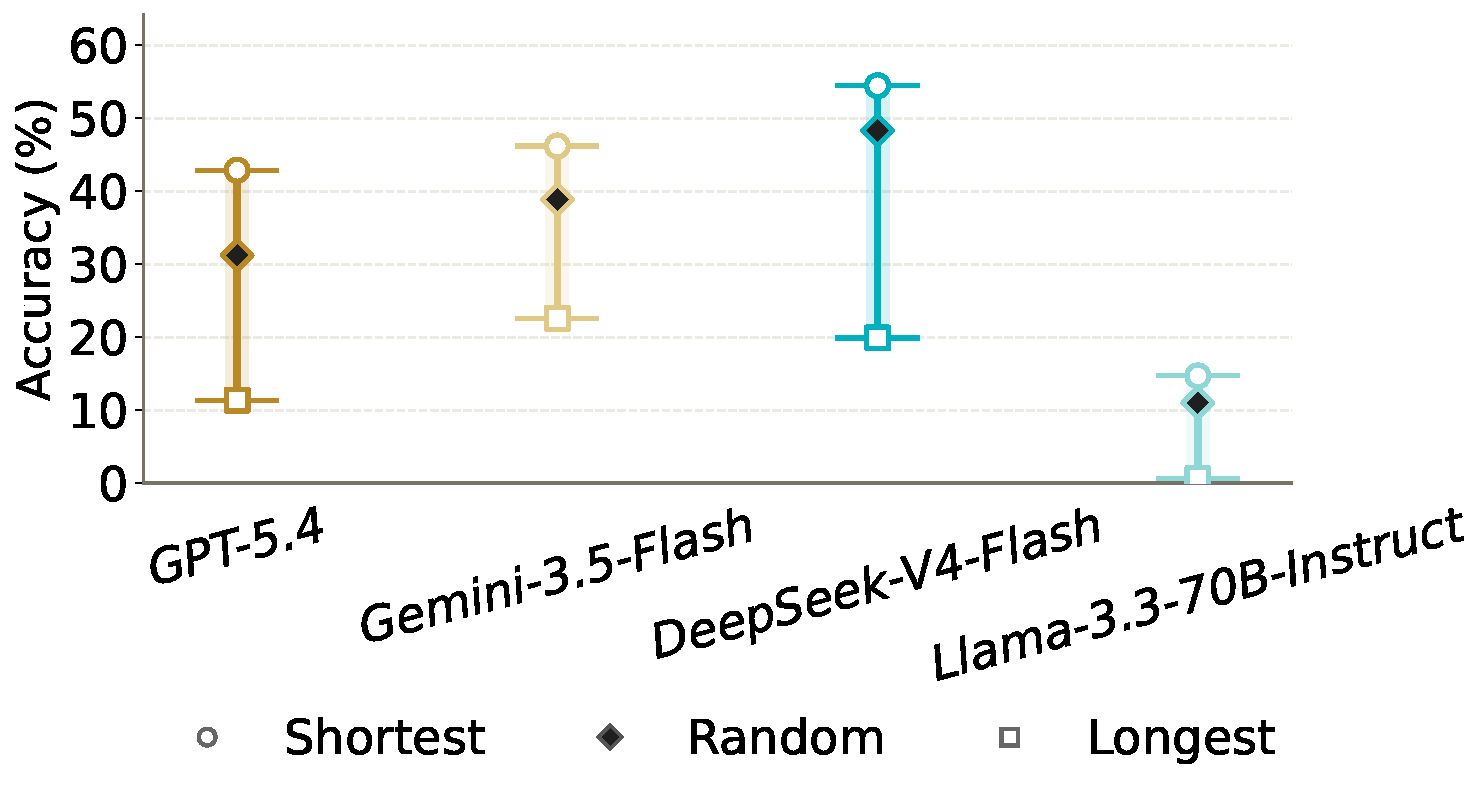
\includegraphics[width=1\linewidth]{Figures/fine_grained_blocking_pdf.pdf}
    \vspace{-0.15in}
    \caption{Accuracy (\%) on \bench{} under fine-grained blocking. \textit{Shortest} and \textit{Longest} denote runs where blocking preserves the shortest and longest admissible solution paths, respectively; \textit{Random} denotes the basic blocked configuration. Circles, squares, and diamonds mark these three settings.}
    \label{fig:fine_grained_blocking}
    \vspace{-0.1in}
\end{figure}